% Dakota study block hierarchy (prototype for docs/user/img/src/)
\documentclass[tikz,border=6pt]{standalone}
\usepackage[T1]{fontenc}
\usepackage{helvet}
\renewcommand{\familydefault}{\sfdefault}
\usetikzlibrary{positioning,fit,arrows.meta}

\definecolor{dakblue}{HTML}{1F5A96}
\definecolor{dakfill}{HTML}{E8F0F8}
\definecolor{envline}{HTML}{8C8C8C}

\begin{document}
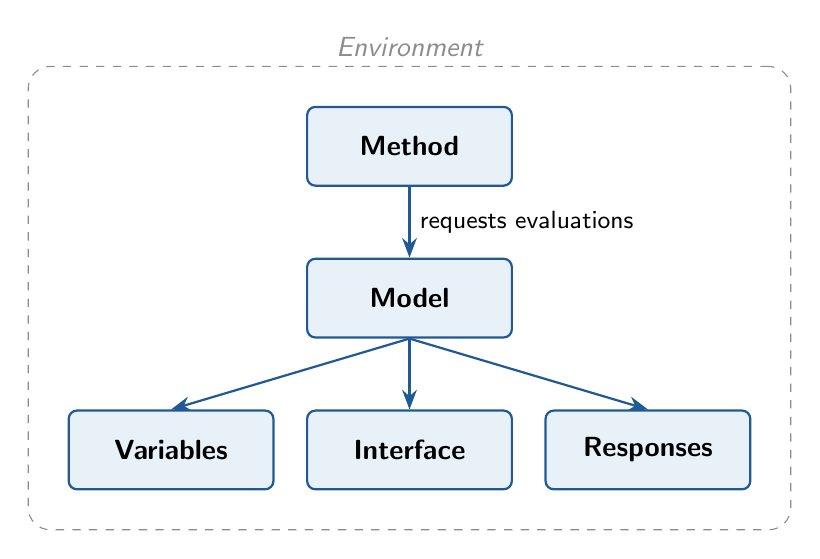
\begin{tikzpicture}[
    blk/.style={draw=dakblue, fill=dakfill, thick, rounded corners=3pt,
                minimum width=26mm, minimum height=10mm, font=\bfseries},
    arr/.style={-{Stealth[length=2.5mm]}, thick, dakblue},
    node distance=9mm and 4mm]

  \node[blk] (method) {Method};
  \node[blk, below=of method] (model) {Model};
  \node[blk, below=of model] (interface) {Interface};
  \node[blk, left=of interface] (variables) {Variables};
  \node[blk, right=of interface] (responses) {Responses};

  \draw[arr] (method) -- node[right, font=\small, text=black]{requests evaluations} (model);
  \draw[arr] (model.south) -- (variables.north);
  \draw[arr] (model) -- (interface);
  \draw[arr] (model.south) -- (responses.north);

  \node[draw=envline, dashed, rounded corners=8pt, inner sep=5mm,
        fit=(method)(variables)(responses),
        label={[font=\itshape, text=envline]above:Environment}] {};
\end{tikzpicture}
\end{document}
